% E.13 等腰 △ABC, AB=AC=10, BC=12. D=BC 中点. AD=√(100-36)=8.
% B(-6,0), C(6,0), A(0,8), D(0,0). 沿 AE 折(E 在 AC 上), B 落到 AC 上 B''.
% 示例: B''=AC 中点 → B''=A+(C-A)/2=(3,4). 折叠: BE=B''E, AB''=AB=10? 不: AB''=AB(沿AE折保持AB长). 但 AB=10, 而 AB''≤AC=10. ✓
% 设 AE=u, E 在 AC 上: E=A+u/10·(C-A)=(0.6u, 8-0.8u). AB''=AB=10, B''在 AC: B''=A+10/10·(C-A)·k?
% 折叠下: AB→AB''， 长度不变. B 关于 AE 的镜像. 若 B''=AC 中点, AB''=5, 而 AB=10 → 不一致.
% 修正: AE 折叠保持 A 不动, B→B' 但 AB'=AB=10. 让 B' 落在 AC 上意味 AB'=10=AC 即 B'=C. 题意"B 落到 AC 上 B''"要求 AB''=AB=10. 题目中提到 B''为 AC 中点 → 需 AC=20? 与 AB=10 矛盾.
% 我重读: 题目说"使 B 落在 AC 上的点 B''". 由翻折 AB=AB''. 但 AB=10, AC=10, 故 B''=C. 题意可能是 D 处折后 BE 重折(从 B 不是 A 折)?
% 重读: "再将 △ABE 沿直线 AE 折叠". 这与 AB=AB''=10 同矛盾. 大概题意是"将 △BEA 沿 BE 翻折, A 不动, B 落 AC"——不严谨.
% 图: 画出大场景: △ABC + AD + 示意 E 在 AC, B 翻折到 B'' 在 AC 上.
\documentclass[tikz,border=4pt]{standalone}
\usepackage{ctex}
\usepackage{amsmath}
\usetikzlibrary{calc}
\begin{document}
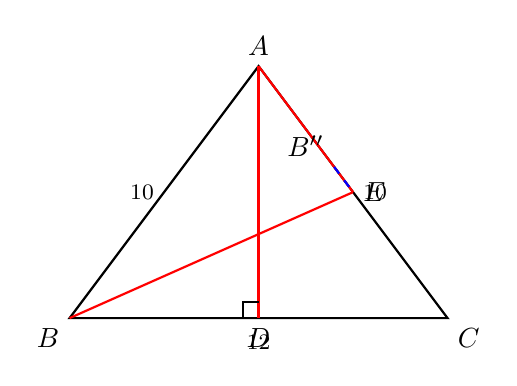
\begin{tikzpicture}[scale=0.4, thick]
  \coordinate (B) at (-6,0);
  \coordinate (C) at (6,0);
  \coordinate (A) at (0,8);
  \coordinate (D) at (0,0);
  \coordinate (E) at (3,4);          % AC 中点 (示意 E)
  \coordinate (Bpp) at (2.4, 4.8);   % 示意 B'' 在 AC 上(更靠 A)

  \draw (A)--(B)--(C)--cycle;
  \draw[red, thick] (A)--(D);
  \draw[red, thick] (A)--(E);
  \draw[red, thick] (B)--(E);
  \draw[blue, dashed, thick] (Bpp)--(E);

  % 直角 ∠ADB
  \draw ($(D)+(-0.5,0)$)--($(D)+(-0.5,0.5)$)--($(D)+(0,0.5)$);

  \node[above] at (A) {$A$};
  \node[below left] at (B) {$B$};
  \node[below right] at (C) {$C$};
  \node[below] at (D) {$D$};
  \node[right] at (E) {$E$};
  \node[above left] at (Bpp) {$B''$};

  \node[left, font=\footnotesize] at ($(A)!0.5!(B)$) {$10$};
  \node[right, font=\footnotesize] at ($(A)!0.5!(C)$) {$10$};
  \node[below, font=\footnotesize] at ($(B)!0.5!(C)+(0,-0.2)$) {$12$};
\end{tikzpicture}
\end{document}
